%-----------------------------------------------------------------------
%                                                                 aa.tex
% AA vers. 9.4, LaTeX class for Astronomy & Astrophysics
% Demonstration file
%                                                       (c) EDP Sciences
%-----------------------------------------------------------------------
%
%\documentclass[referee]{aa}    % for a referee version
%\documentclass[onecolumn]{aa}  % for a paper on 1 column  
%\documentclass[longauth]{aa}   % for long lists of authors and/or affiliations. 
                                % This command displays the first eight authors on page 1
                                % and shift the whole list after the references.
                                % Ensure to separate each author with the \and command (see below)
%\documentclass[letter]{aa}     % for the letters
%\documentclass[bibyear]{aa}    % if the references are not structured
                                % according to the author-year natbib style

\documentclass{aa}  
\usepackage{natbib}

\usepackage{graphicx}
\usepackage{txfonts}
\usepackage{subcaption}         % necessary for continued figures, example in section 3
                                % and appendix
\usepackage{lscape}             % to rotate a single page table, example in appendix.
                                % For landscape tables, see the longtable examples.
\usepackage{placeins}           % useful with \FloatBarrier, to keep 
                                % onecolumn floats from drifting to the next section
                                

\usepackage[hidelinks]{hyperref}


%%%%%%%%%%%%%%%%%%%%%%%%%%%%%%%%%%%%%%%%
% LINKS

\newcommand{\Molecfit}{\href{https://www.eso.org/sci/software/pipelines/skytools/molecfit}{Molecfit }}

\newcommand{\LBLRTM}{\href{https://github.com/AER-RC/LBLRTM}{LBLRTM }}

\newcommand{\GDAS}{\href{https://psl.noaa.gov}{GDAS }}

\newcommand{\HITRAN}{\href{https://hitran.org}{HITRAN }}

\newcommand{\MIPAS}{\href{https://earth.esa.int/eogateway/instruments/mipas}{MIPAS }}

\newcommand{\pymolfit}{PyMolFit }

%%%%%%%%%%%%%%%%%%%%%%%%%%%%%%%%%%%%%%%%


\begin{document}

%%%%%%%%%%%%%%%%%%%%%%%%%%%%%%%%%%%%%%%%
% if you use custom commands in your title,
% ensure to check your title when submitting!
%%%%%%%%%%%%%%%%%%%%%%%%%%%%%%%%%%%%%%%%
   \title{PyMolFit: A pure-Python framework for model-based telluric correction}

   \subtitle{}

%%%%%%%%%%%%%%%%%%%%%%%%%%%%%%%%%%%%%%%%
% Please separate each author with the \and command
%
% Use the \corrauth to provide the corresponding
% author address. It will be automatically inserted as 
% footnote in the PDF output.
%
% Please DO NOT include ORCIDs next to author names.
% Instead, please provide an active address for each coauthor:
% it will be automatically extracted by EDPS editorial system, 
% and co-authors will be be able to authenticate their ORCID.
%
% Only authenticated ORCIDs will be taken into account.
% ORCIDs included here will be removed.
%%%%%%%%%%%%%%%%%%%%%%%%%%%%%%%%%%%%%%%%

   \author{N. Valsamidis\inst{1}\corrauth{nikolasvalsamidis97@gmail.com}        % use \corrauth for the corresponding author
        \and A. Brandeker\inst{1}\email{alexis@astro.su.se}
        }

   \institute{Stockholm University, 11421, Stockholm, Sweden}

   \date{Received September 30, 20XX}

% \abstract{}{}{}{}{}
% 5 {} token are mandatory
 
  \abstract
  % context heading (optional)
  % {} leave it empty if necessary  
   {}
  % aims heading (mandatory)
   {} 
  % methods heading (mandatory)
   {}
  % results heading (mandatory)
   {}
  % conclusions heading (optional), leave it empty if necessary
   {}

   \keywords{}

   \maketitle


%%%%%%%%%%%%%%%%%%%%%%%%%%%%%%%%%%%%%%%%%%%%%%%%%%%%%%%%%%%%%%%%%%%%%%%%%%%%%%%%
% 1 Introduction
%%%%%%%%%%%%%%%%%%%%%%%%%%%%%%%%%%%%%%%%%%%%%%%%%%%%%%%%%%%%%%%%%%%%%%%%%%%%%%%%

\section{Introduction}

Ground-based astronomical spectra are affected by absorption in the Earth’s atmosphere. These telluric absorption features contaminate the observed spectrum and can interfere with the detection and analysis of astrophysical spectral lines, particularly when stellar and atmospheric features overlap in wavelength. Accurate modelling and correction of telluric absorption is therefore an essential step in the reduction and interpretation of many spectroscopic observations.

[Why empirical telluric correction / standard stars can be problematic]

[Model-based telluric correction and the role of Molecfit]



%%%%%%%%%%%%%%%%%%%%%%%%%%%%%%%%%%%%%%%%%%%%%%%%%%%%%%%%%%%%%%%%%%%%%%%%%%%%%%%%
% 2 PyMolFit
%%%%%%%%%%%%%%%%%%%%%%%%%%%%%%%%%%%%%%%%%%%%%%%%%%%%%%%%%%%%%%%%%%%%%%%%%%%%%%%%

\section{PyMolFit framework}

\pymolfit implements the model-based telluric-correction approach used by \Molecfit\ \citep{MOLECFIT1,MOLECFIT2} in Python, with assistance from AI coding tools during development. Parameter fitting, calculation of atmospheric transmission over the full spectral range, and application of the telluric correction are combined into a single function, \texttt{correct()}. This function accepts spectrum files, loaded spectrum objects, or wavelength--flux arrays and returns the corrected spectrum together with the fitted transmission, model parameters, masks, and diagnostic information.

PyMolFit automatically divides the spectrum into smaller processing segments while preserving spectral-order and detector-group boundaries. Fitting regions can be selected automatically or defined and edited through an interactive selector. When a theoretical stellar spectrum is supplied, PyMolFit uses it to identify stellar features and exclude the corresponding wavelength regions from telluric parameter estimation. These exclusions affect only the fit: atmospheric transmission is still calculated in the excluded regions when applying the correction.

The atmospheric modelling follows established physical methods rather than introducing a new formalism. However, whereas \Molecfit uses \LBLRTM for its radiative-transfer calculations \citep{MOLECFIT1}, PyMolFit evaluates atmospheric absorption through its own numerical implementation, without executing either program. Differences in numerical implementation and optimisation can therefore produce different transmission spectra and fitted parameters. These differences are assessed in Sect.~\ref{sec:validation}.


%%%%%%%%%%%%%%%%%%%%%%%%%%%%%%%%%%%%%%%%%%%%%%%%%%%%%%%%%%%%%%%%%%%%%%%%%%%%%%%%
% 3 Methodology
%%%%%%%%%%%%%%%%%%%%%%%%%%%%%%%%%%%%%%%%%%%%%%%%%%%%%%%%%%%%%%%%%%%%%%%%%%%%%%%%

\section{Methodology}

\subsection{Atmospheric profile and absorption calculation}

PyMolFit follows the atmospheric-profile construction used by \Molecfit\ \citep{MOLECFIT1}, combining a MIPAS reference atmosphere \citep{MIPAS_PROFILE} with GDAS pressure, temperature, and water-vapour profiles \citep{GDAS}. Conditions at the observation time are estimated from a time-weighted average of the bracketing GDAS profiles. When these are unavailable, PyMolFit uses the same two-month average profiles as Molecfit. Available local weather measurements adjust the lowest layers. The molecular number density at altitude \(h\) is
\begin{equation}
    n_s(h) = x_s(h)\,\frac{P(h)}{k_{\mathrm B}T(h)},
\end{equation}
where \(x_s\) is the number fraction of species \(s\), \(P\) and \(T\) are pressure and temperature, and \(k_{\mathrm B}\) is Boltzmann's constant. The line-of-sight column density through layer \(i\) is
\begin{equation}
    N_{s,i} = \int_{\mathcal{L}_i} n_s[h(\ell)]\,\mathrm{d}\ell,
\end{equation}
where \(\mathcal{L}_i\) is the light path within the layer and \(\ell\) measures distance along it. The path is calculated from the observation airmass, supplied explicitly or read from metadata, accounting for spherical geometry and atmospheric refraction.

Absorption is evaluated on a grid finer than the detector sampling. The AER catalogue \citep{AER} supplies line positions, integrated strengths \(S_j(T_{\mathrm{ref}})\), and broadening parameters at \(T_{\mathrm{ref}}=296\,\mathrm{K}\) \citep{HITRAN}. For transition \(j\) in layer \(i\), the cross-section at wavenumber \(\tilde{\nu}=1/\lambda\), where \(\lambda\) is wavelength, is
\begin{equation}
    \sigma_{j,i}(\tilde{\nu}) = S_j(T_i)\,\phi_{j,i}(\tilde{\nu}).
\end{equation}
Here, \(S_j(T_i)\) is the strength adjusted to the layer temperature \(T_i\), and \(\phi_{j,i}\) is the effective Voigt-based profile. Local pressure, temperature, and composition determine the line position and Doppler and collisional broadening. The default treatment, \texttt{lblrtm\_panel}, implements LBLRTM-style accumulation on nested grids, with line-dependent profile limits and a separate far-wing contribution extending to \(25\,\mathrm{cm}^{-1}\) from line centre. These effective profiles need not retain unit-area normalisation. The discrete-line optical depth is
\begin{equation}
    \tau_{\mathrm{lines}}(\tilde{\nu}) = \sum_i\sum_s N_{s,i}\sum_{j\in s}\sigma_{j,i}(\tilde{\nu}),
\end{equation}
where \(j\in s\) denotes transitions of species \(s\). Enabled atmospheric continuum contributions, including water-vapour and carbon-dioxide absorption, give an additional optical depth \(\tau_{\mathrm{cont}}\) \citep{MTCKD,LBLRTM}. The total optical depth and Beer--Lambert transmission are \citep{RYBICKI1979}
\begin{equation}
    \begin{aligned}
        \tau_{\mathrm{atm}}(\tilde{\nu}) &= \tau_{\mathrm{lines}}(\tilde{\nu})+\tau_{\mathrm{cont}}(\tilde{\nu}),\\
        T_{\mathrm{atm}}(\tilde{\nu}) &= \exp[-\tau_{\mathrm{atm}}(\tilde{\nu})].
    \end{aligned}
\end{equation}

\subsection{Spectral segmentation and fit-region selection}
\begin{figure*}[t]
    \centering
    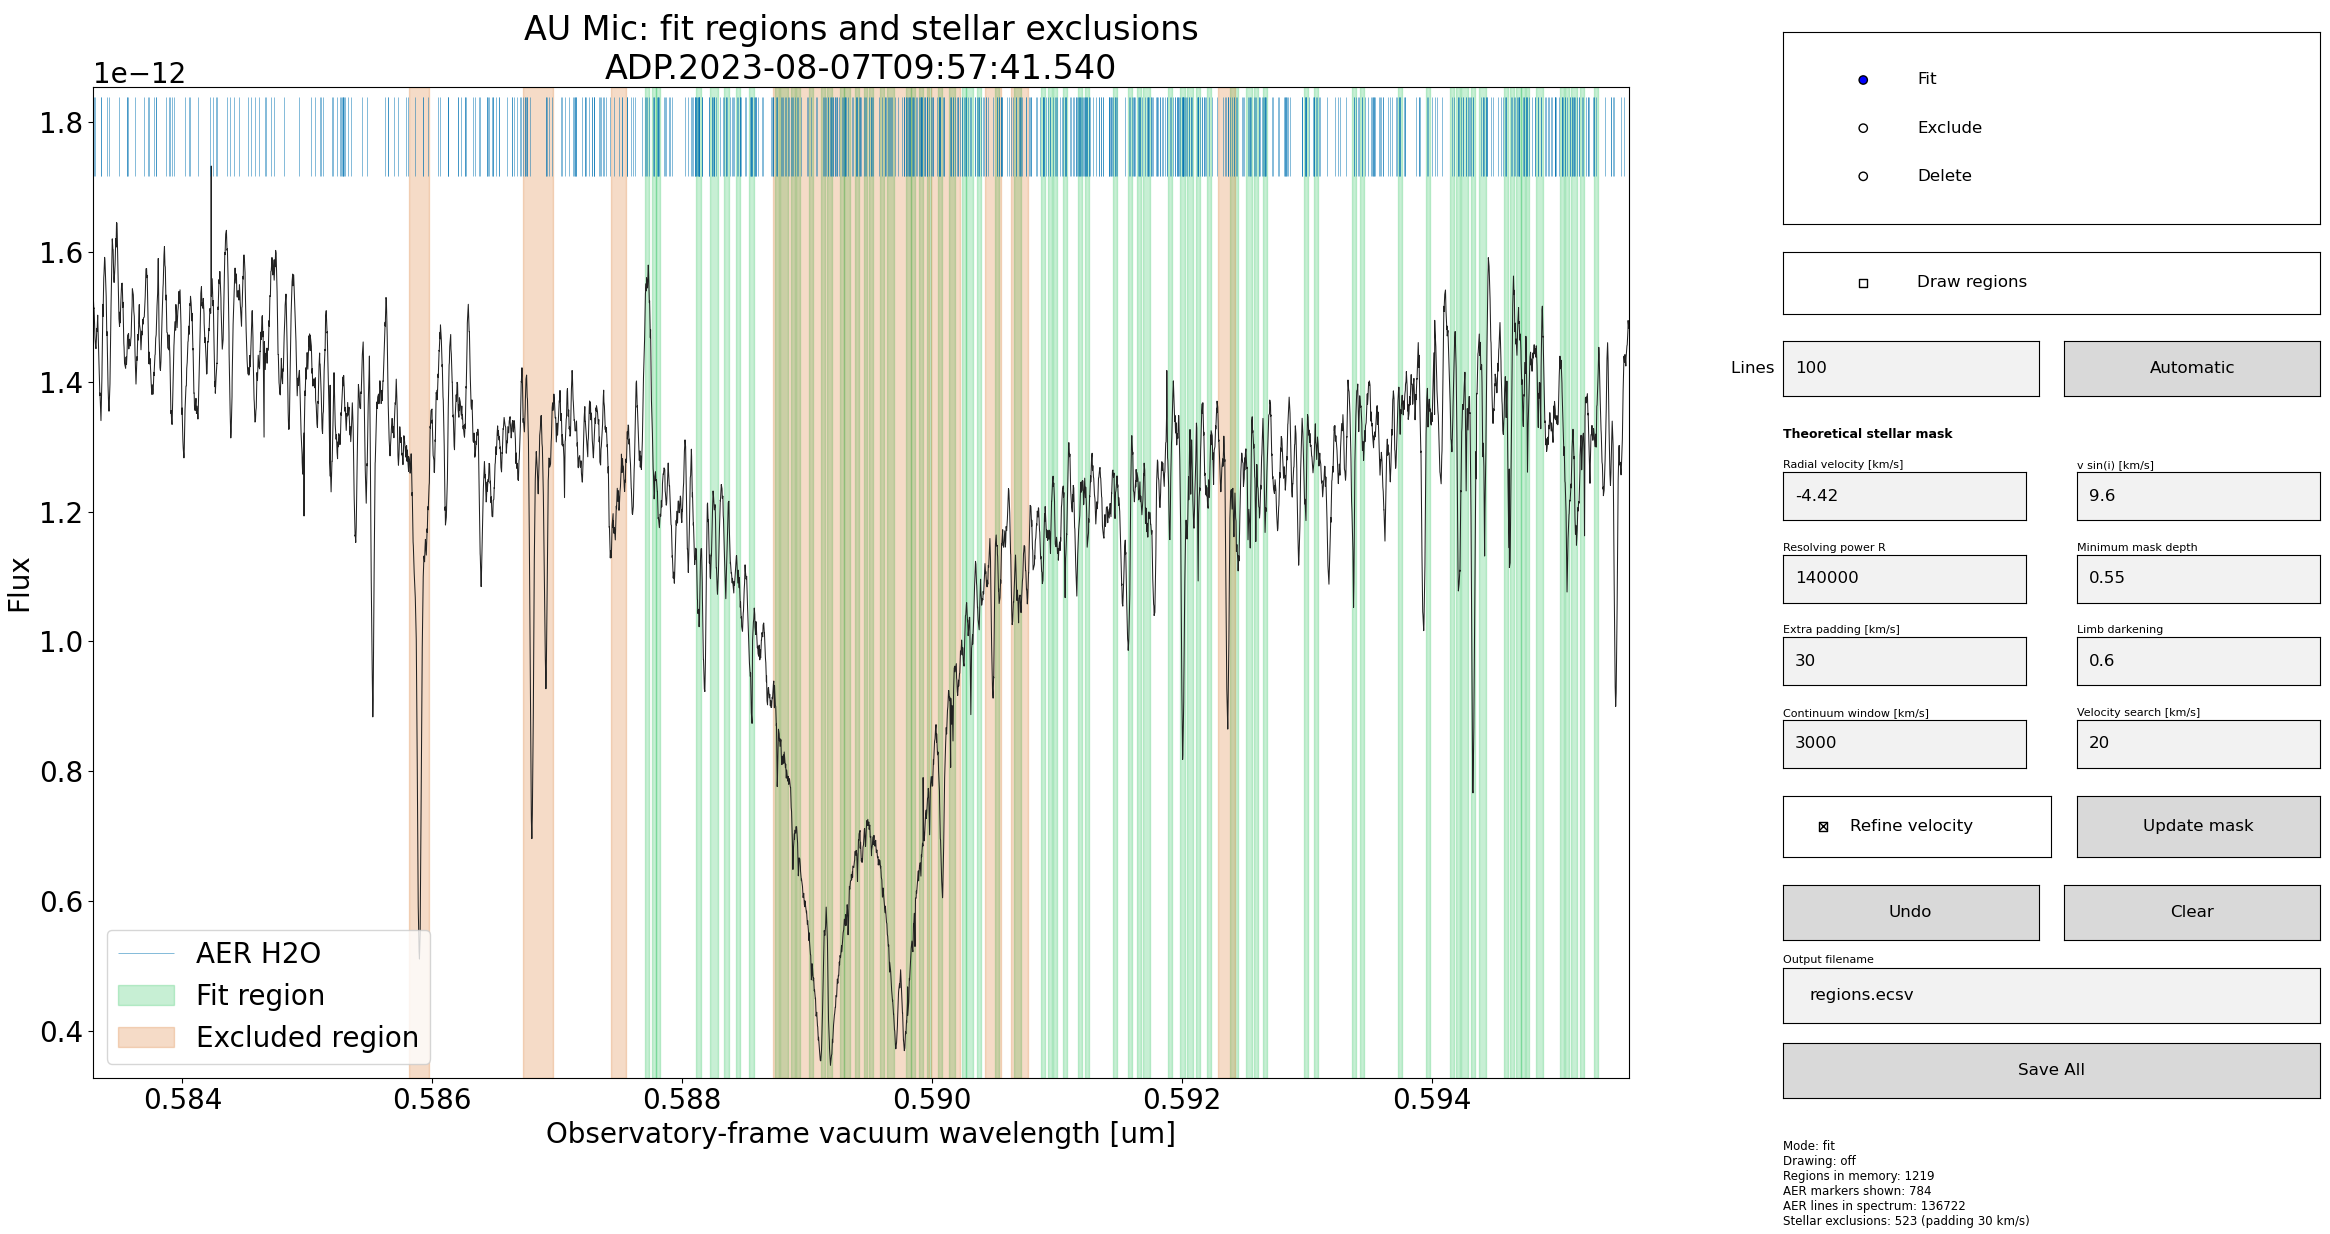
\includegraphics[width=\textwidth]{Images/Interactive_selector.png}
    \caption{PyMolFit's interactive region selector around the AU Mic Na\,I D doublet. Green and orange shading mark fitting and stellar exclusion intervals; exclusions take precedence where they overlap. The controls allow manual editing and adjustment of line-selection and stellar-template settings. Blue ticks mark H$_2$O transitions from the AER catalogue.}
    \label{fig:Interactive_selector}
\end{figure*}
PyMolFit divides the spectrum into processing segments while preserving spectral-order and detector-group boundaries, identified from metadata or inferred from large wavelength gaps. The default target width is 50\,\AA, with further subdivision if the atmospheric grid exceeds two million points per segment. These configurable limits control memory use without coarsening the model grid.

Fitting and exclusion intervals can be supplied directly or edited in the interactive selector (Fig.~\ref{fig:Interactive_selector}). They select the observed pixels used to constrain molecular columns, wavelength corrections, continuum parameters, and instrumental broadening. Automatic fitting-region selection ranks AER transitions within the observed coverage by
\begin{equation}
    A_j = S_j(T_{\mathrm{ref}})\,N_{s(j),\mathrm{rep}},
\end{equation}
where \(s(j)\) identifies the species of transition \(j\), and \(N_{s(j),\mathrm{rep}}\) is its column density in a fixed reference atmosphere. Intervals of configurable half-width in detector pixels are placed around the requested number of highest-scoring lines and merged where they overlap.

Exclusions remove stellar features or defective pixels from the fit. For automatic stellar exclusions, PyMolFit continuum-normalises a theoretical spectrum and applies rotational broadening. Instrumental broadening uses a supplied or metadata-derived resolving power when available, not the subsequently fitted instrumental profile. The template is converted to the observation's wavelength medium and reference frame using the stellar radial velocity and observation frame correction, with optional residual alignment by cross-correlation. Template pixels exceeding a configurable fractional deviation from the continuum are grouped into exclusions and extended by velocity padding. These exclusions remain fixed during fitting unless regenerated.

Only valid pixels inside fitting intervals and outside exclusions contribute to parameter estimation. If no fitting intervals are specified, all valid, non-excluded pixels are used.

\subsection{Spectral modelling and parameter estimation}
PyMolFit fits a model of the observed flux to these selected pixels. Molecular column-density scales initially equal unity relative to the atmospheric profile. Initial wavelength alignment follows the input calibration and metadata-based frame correction. The initial Gaussian instrumental width is estimated from resolving-power metadata and detector sampling, or from narrow observed features when this information is unavailable. User-supplied starting values can replace these estimates.

For each trial, the high-resolution atmospheric transmission receives a constant or polynomial wavelength correction. In the default implementation, transmission is averaged over each observed pixel's wavelength interval, accounting for partial overlap at pixel boundaries, then convolved with the normalised instrumental line-spread function. Only the model is resampled; the observation remains unchanged. The resulting \(\widehat T_{kp}\) includes wavelength correction, detector sampling, and instrumental broadening at pixel \(p\) in segment \(k\). The instrumental profile supports Gaussian, Lorentzian, and boxcar components, with optional wavelength-dependent widths.

A local polynomial continuum represents the smooth flux level, distinct from the atmospheric continuum absorption included in \(\tau_{\mathrm{cont}}\). The predicted flux is
\begin{equation}
    C_{kp} = \sum_{m=0}^{d}c_{km}u_{kp}^{m}, \qquad F^{\mathrm{mod}}_{kp} = C_{kp}\,\widehat T_{kp},
\end{equation}
where \(c_{km}\) is the coefficient of term \(m\) in segment \(k\), \(d\) is the continuum polynomial order, and \(u_{kp}\) maps wavelength linearly from \(-1\) to \(+1\) across the segment. The default \(d=1\) gives a linear continuum. The default fit minimises
\begin{equation}
    \chi^2 = \sum_k\sum_{p\in\mathcal F_k}\left[\frac{F^{\mathrm{obs}}_{kp}-F^{\mathrm{mod}}_{kp}}{\sigma_{F,kp}}\right]^2,
\end{equation}
where \(F^{\mathrm{obs}}_{kp}\) and \(\sigma_{F,kp}\) are the observed flux and its uncertainty, and \(\mathcal F_k\) contains the selected fitting pixels in segment \(k\). Without supplied uncertainties, fitting uses a constant error of one percent of the mean observed flux in each segment's fitted pixels. Robust loss functions are optional.

Bounded trust-region reflective least squares adjusts the molecular scales and enabled wavelength and instrumental parameters, recalculating the model at each trial. Molecular scales are fitted logarithmically and shared across segments; atmospheric pressure and temperature profiles remain fixed. Wavelength corrections defined per order or detector group are shared across its segments. Continuum coefficients are independent between segments and normally solved by linear least squares at each trial.

Convergence requires sufficiently small relative objective improvement, parameter steps, or scaled gradient, with default tolerances \texttt{ftol} = \texttt{xtol} = \texttt{gtol} = \(10^{-10}\). A model-evaluation limit can also terminate fitting without convergence.

\subsection{Corrected spectrum and uncertainty propagation}
The best-fitting transmission is evaluated over the full input coverage, including excluded regions and wavelengths outside the fitting intervals. The corrected flux is
\begin{equation}
    F^{\mathrm{corr}}_{kp} = \frac{F^{\mathrm{obs}}_{kp}}{\widehat T_{kp}}.
\end{equation}
The continuum is not divided out. Invalid pixels and pixels with transmission below a configurable threshold, 0.01 by default, are masked.

Optional transmission uncertainties \(\sigma_{T,kp}\) are obtained by propagating the local fitted-parameter covariance through the transmission model using numerical derivatives. The covariance is scaled by the reduced chi-square; rank-deficient estimates are flagged as unavailable. Neglecting covariance between the observed flux and fitted transmission, the corrected-flux variance is
\begin{equation}
    \sigma^2_{F^{\mathrm{corr}},kp} \simeq \frac{\sigma_{F,kp}^{2}}{\widehat T_{kp}^{2}} + \frac{\left(F^{\mathrm{obs}}_{kp}\right)^2}{\widehat T_{kp}^{4}}\,\sigma_{T,kp}^{2}.
\end{equation}
Only supplied flux uncertainties are propagated by default. Optional transmission-uncertainty propagation is limited to segments participating in the fit. These statistical estimates exclude systematic errors in the atmospheric profiles, spectroscopic data, and model assumptions.

%%%%%%%%%%%%%%%%%%%%%%%%%%%%%%%%%%%%%%%%%%%%%%%%%%%%%%%%%%%%%%%%%%%%%%%%%%%%%%%%
% 5 Validation
%%%%%%%%%%%%%%%%%%%%%%%%%%%%%%%%%%%%%%%%%%%%%%%%%%%%%%%%%%%%%%%%%%%%%%%%%%%%%%%%

\section{Validation}\label{sec:validation}

\subsection{Component-level physical validation}

\subsection{Synthetic data}

% Demonstrate recovery of known parameters.

\subsection{Comparison with Molecfit and LBLRTM}

% Compare results.
%
% Demonstrate agreement where expected.

\subsection{Example application}

% Demonstrate PyMolFit on real observational data.


%%%%%%%%%%%%%%%%%%%%%%%%%%%%%%%%%%%%%%%%%%%%%%%%%%%%%%%%%%%%%%%%%%%%%%%%%%%%%%%%
% 6 Discussion
%%%%%%%%%%%%%%%%%%%%%%%%%%%%%%%%%%%%%%%%%%%%%%%%%%%%%%%%%%%%%%%%%%%%%%%%%%%%%%%%

\section{Discussion}
% Planned future developments:
% stronger Molecfit/LBLRTM parity,
% broader continuum support,
% and further validation of the joint stellar model.


%%%%%%%%%%%%%%%%%%%%%%%%%%%%%%%%%%%%%%%%%%%%%%%%%%%%%%%%%%%%%%%%%%%%%%%%%%%%%%%%
% 7 Availability
%%%%%%%%%%%%%%%%%%%%%%%%%%%%%%%%%%%%%%%%%%%%%%%%%%%%%%%%%%%%%%%%%%%%%%%%%%%%%%%%

\section{Software and data availability}

% Repository.
%
% License.
%
% Installation.
%
% Documentation.


%%%%%%%%%%%%%%%%%%%%%%%%%%%%%%%%%%%%%%%%%%%%%%%%%%%%%%%%%%%%%%%%%%%%%%%%%%%%%%%%
% 8 Conclusions
%%%%%%%%%%%%%%%%%%%%%%%%%%%%%%%%%%%%%%%%%%%%%%%%%%%%%%%%%%%%%%%%%%%%%%%%%%%%%%%%

\section{Conclusions}

% Summarize:
%
% Motivation
% Main capabilities
% Validation
% Availability
%
% End with the future outlook.


\begin{acknowledgements}

\end{acknowledgements}




%%%%%%%%%%%%%%%%%%%%%%%%%%%%%%%%%%%%%%%%%%%%%%%%%%%%%%%%%%%%%%
% WARNING
% Please note that we have included the references below in
% order to compile the document, but we ask you to:
%
% - use BibTeX with the regular commands:
%   \bibliographystyle{aa} % style aa.bst
%   \bibliography{Yourfile} % your references Yourfile.bib
% - join the .bib files when you upload your source files
%%%%%%%%%%%%%%%%%%%%%%%%%%%%%%%%%%%%%%%%%%%%%%%%%%%%%%%%%%%%%%

\bibliographystyle{aa}
\bibliography{bibliography}

\end{document}